
\chapter{ಗ್ರೇಟ್​ ಟ್ರಿಗನಮಿಟ್ರಿಕಲ್​ ಸರ್ವೇಯ ಹೆಗ್ಗುರುತು ಅದರ ಶ್ರೇಷ್ಠ ನಿಖರತೆ}

\vskip -8pt

ಗ್ರೇಟ್​ ಟ್ರಿಗನಮಿಟ್ರಿಕಲ್​ ಸರ್ವೇ ತಂಡದ ಸಾಧನೆಯು ಬಹು ರೋಚಕವಾದದ್ದು. ಅದು ವಿಜ್ಞಾನದ ವಿಜಯ, ವಿಜ್ಞಾನದ ವೈಭವ. ಭಾರತದ ಉಪಖಂಡದ \enginline{2400} ಕಿಲೋಮೀಟರ್​ ಉದ್ದಗಲಕ್ಕೆ ಸಾಗಿದ ಮಹಾಸರ್ವೇ. ಬಾರೀ ಗಾತ್ರದ, ಸಾಟಿ ಇಲ್ಲದ ವಿಜ್ಞಾನ ಮಹಾಸಾಧನೆ ಅದು. ಏಕೆಂದರೆ ಅತ್ಯಂತ ಶ್ರಮದಾಯಕವಾದ, ಈ ಗ್ರೇಟ್​ ಟ್ರಿಗನಮಿಟ್ರಿಕಲ್​ ಸರ್ವೇಯ ಹೆಗ್ಗುರುತು ಎಂದರೆ ಅದರ ಅತೀ ಶ್ರೇಷ್ಠ ನಿಖರತೆ. ಗ್ರೇಟ್​ ಟ್ರಿಗನಮಿಟ್ರಿಕಲ್​ ಸರ್ವೇಯಲ್ಲಿ ಜಿಯೋಡೆಸಿ, ಮ್ಯಾಥಮೆಟಿಕ್ಸ್​, ಅಸ್ಟ್ರನಮಿ ಮತ್ತು ಸರ್ವೇಯಿಂಗ್​ ವಿಷಯಗಳು ಒಂದಕ್ಕೊಂದು ಸಂಬಂಧಿಸಿವೆ. ಒಂದನೊಂದು ಅವಲಂಬಿಸಿವೆ. ಅರ್ಧ ಶತಮಾನಕ್ಕೂ ಮೀರಿ ನಡೆದ ಈ ವೈಜ್ಞಾನಿಕ ಮಹಾಕಾರ್ಯ ನಡೆದದ್ದು ನಾಲ್ಕು ಗೋಡೆಗಳ ನಡುವಿನ ಪ್ರಯೋಗಾಲಯದಲ್ಲಿ ಅಲ್ಲ. ಆ ಕಾರ್ಯಾಚರಣೆ ನಡೆದದ್ದು ಹೊರಗಿನ ತೆರೆದ ವಿಶಾಲ ಬಯಲಿನಲ್ಲಿ. ದುರ್ಗಮ ಕಾಡಿನಲ್ಲಿ. ಸುರಿಯುವ ಮಳೆಯಲ್ಲಿ. ಸುಡುವ ಬಿಸಿಲಿನಲ್ಲಿ. ಆದ್ದರಿಂದ ಈ ವೈಜ್ಞಾನಿಕ ಮಹಾ ಕಾರ್ಯದಲ್ಲಿ ಆದ ಕಷ್ಟ ನಷ್ಟ ಜೀವ ಹಾನಿ ಅಪಾರ.

ಈ ಮ್ಯಾಪಿಂಗ್​ ಕಾರ್ಯವು ಇಂಚು ನಿಖರತೆಯ ಅತಿ ಶ್ರೇಷ್ಠ ನಕ್ಷಾ ರಚನಾ ಕಾರ್ಯವೆಂದೇ ಪ್ರಸಿದ್ಧಿ ಪಡೆದಿದೆ. ಈ ಸರ್ವೇ ಕಾರ್ಯಾಚರಣೆಯ ನಿಖರತೆಯ ಮಟ್ಟವು, ಲಭ್ಯ ಇರುವ ಇಂದಿನ \enginline{21}ನೇ ಶತಮಾನದ ಆಧುನಿಕ ಉಪಕರಣ, ತಂತ್ರಜ್ಞಾನಗಳನ್ನು ಬಳಸಿ ಮಾಡುವ ಸರ್ವೇ ಕಾರ್ಯಕ್ಕೆ ಸಮ ಸಮ ಆಗಿರುವಂತಹ ಶ್ರೇಷ್ಠ ಕಾರ್ಯವಾಗಿದೆ. ಈ ಮಹಾ ಕಾರ್ಯವನ್ನು ‘19ನೇ ಶತಮಾನದ ವಿಜ್ಞಾನದ ಪ್ರಗತಿಗೆ ಮಹಾ ಕೊಡುಗೆ’ ಎಂದು ರಾಯಲ್​ ಜೀಯೋಗ್ರಫಿಕ್​ ಸೊಸೈಟಿಯು ಸರಿಯಾಗಿಯೇ ಕರೆದಿದೆ.

ಲ್ಯಾಂಬ್​ಟನ್​ರವರು ಟ್ರೈಯಾಂಗ್ಯುಲೇಷನ್​ ಕಾರ್ಯವನ್ನು ಪೂರ್ವದ ಮದರಾಸಿನ ಕಡಲ ತೀರದಿಂದ, ಗುಡ್ಡ ಬೆಟ್ಟ ಕಾಡು ಮೇಡು ದಾಟಿ, ಪಶ್ಚಿಮದ ಮಂಗಳೂರಿನ ಕಡಲ ತೀರದೆಡೆಗೆ ನಿಧಾನವಾಗಿ ಸಾಗಿಸಿದರು. ಮಧ್ಯದಲ್ಲಿ ಮದ್ರಾಸ್​ನಿಂದ ಪಶ್ಚಿಮಕ್ಕೆ, \enginline{200} ಮೈಲು ದೂರದ ಬೆಂಗಳೂರನ್ನು \enginline{1804} ರಲ್ಲಿ ತಲುಪಿದರು. ಸುಮಾರು \enginline{200} ಮೈಲು ದೂರವನ್ನು ಟ್ರೈಯಾಂಗ್ಯುಲೇಷನ್​ ಕಾರ್ಯವು ಈಗಾಗಲೇ ಸಾಗಿಬಂದಿರುವುದರಿಂದ, ಸೂಕ್ತವೆನ್ನುವ ಸ್ಥಳದಲ್ಲಿ ಟ್ರೈಯಾಂಗ್ಯುಲೇಷನ್​ ಕಾರ್ಯದ ನಿಖರತೆಯನ್ನು ಪರಿಶೀಲಿಸಬೇಕಾಗುತ್ತದೆ. ಬೇಸ್‌ಲೈನ್​ ಅಳತೆಯ ಎಲ್ಲಾ ವಿಧಿ ವಿಧಾನಗಳೊಂದಿಗೆ, ಬೆಂಗಳೂರು ಪರಿಶೀಲನಾ ಬೇಸ್‌ಲೈನ್​ ಅಳತೆ ಕಾರ್ಯವನ್ನು ಪ್ರಾರಂಭಿಸಲಾಯಿತು. ಬೆಂಗಳೂರಿನ ಬೇಸ್‌ಲೈನಿನ ಉದ್ದ \enginline{7.19} ಮೈಲುಗಳು. ಇದರ ಅಳತೆಗೆ \enginline{49} ದಿನ ತೆಗೆದುಕೊಂಡಿತು. ಟ್ರೈಯಾಂಗ್ಯುಲೇಷನ್​ ಅಳತೆಗೂ, ನೆಲದ ಮೇಲೆ ಅದನ್ನು ನೇರವಾಗಿ ಅಳೆದಾಗ ದೊರೆತ ಅಳತೆಗೂ ಕೇವಲ \enginline{3.7} ಅಂಗುಲ ವ್ಯತ್ಯಾಸ ಬಂದಿತು. ಇದಾದ ನಂತರ ಬೆಂಗಳೂರಿನ ಸಮೀಪದ ಸಾವನ್​ ದುರ್ಗದಿಂದ ಶ್ರವಣಬೆಳಗೊಳ ಸಮೀಪದ ಮುಳ್ಳಪ್ಪನ್ನಬೆಟ್ಟ ಸ್ಟೇಷನ್​ಗೆ ವೀಕ್ಷಣೆಯನ್ನು ಮಾಡಲಾಯಿತು. ಈ ತಾಣಗಳ ನಡುವಿನ ದೂರವು \enginline{50} ಮೈಲು. ಇದು ಇಡೀ ಟ್ರೈಯಾಂಗ್ಯುಲೇಷನ್​ ಕಾರ್ಯದಲ್ಲಿಯೇ ಒಂದು ದೊಡ್ಡ ತ್ರಿಭುಜದ ಬಾಹುವಾಗಿದೆ.

\vskip 5pt

ಬ್ರಿಟೀಷರು ಅವರ ಸಾಮ್ರಾಜ್ಯ ವಿಸ್ತರಣೆಯ ಜೊತೆಗೆ, ಇಲ್ಲಿನ ಸಸ್ಯ ಸಂಪತ್ತಿನ ಬಗ್ಗೆ ಮತ್ತು ಖನಿಜ ಸಂಪತ್ತಿನ ಬಗ್ಗೆ ಅಪಾರ ಆಸಕ್ತಿ ಹೋದಿದ್ದರು. ಈ ಸಂಪತ್ತಿನ ಅನ್ವೇಷಣೆಗೆ ಶೋಧನೆಗೆ ಅವರಿಗೆ ಸರ್ವೇ ಕಾರ್ಯಾಚರಣೆಯು ಸದಾವಕಾಶವನ್ನು ಒದಗಿಸಿತ್ತು. ಒಂದು ಉದಾಹರಣೆಯನ್ನು ನೋಡಿ. ಲೆಫ್ಟಿನೆಂಟ್​ ಹೆನ್ರಿ ಕೇಟರ್​ರವರು \enginline{1803} ರಲ್ಲಿ ಲ್ಯಾಂಬಟನ್​ರವರಿಗೆ ಸಹಾಯಕರಾಗಿ ಗ್ರೇಟ್​ ಟ್ರಿಗನಮಿಟ್ರಿಕಲ್​ ಸರ್ವೇಯನ್ನು ಸೇರಿದ್ದರು. ಇವರು ಲ್ಯಾಂಬಟನ್​ ರವರಿಗೆ ಸರ್ವೇ ಕ್ಷೇತ್ರದಲ್ಲಿ ಸಹಾಯಕರಾಗಿ ದುಡಿಯುತಿದ್ದಂತಹ ಒಬ್ಬ ಬಹುಮುಖಿ ಪ್ರತಿಭಾವಂತರಾಗಿದ್ದರು. ‘ಉಬಿನಾ ಹುಲ್ಲು’ ಕರ್ನಾಟಕದ ದಕ್ಷಿಣ ಭಾಗದಲ್ಲಿ ಹೇರಳವಾಗಿ ಬೆಳೆಯುವ ಹುಲ್ಲಿನ ಒಂದು ಪ್ರಬೇಧ. ತಮಿಳಿನಲ್ಲಿ ಇದನ್ನು ‘ಎರುದೂವಾಲು ಪಿಲ್ಲು’ ಎಂದು ಕರೆಯುತ್ತಾರೆ. ಇದರ ಬೀಜವು ತೇವಾಂಶಕ್ಕೆ ತೀವ್ರವಾದ ಸಂವೇಧನಾಶೀಲ ಗುಣವನ್ನು ಹೊಂದಿದೆ. ಇದರ ಈ ಗುಣ ವಿಶೇಷವು ಹೆನ್ರಿ ಕೇಟರ್​ರವರ ಗಮನಕ್ಕೆ ಬರುತ್ತದೆ. ಅವರು ಈ ಬೀಜವನ್ನು ಬಳಸಿಕೊಂಡು ಹೈಗ್ರೋಮೀಟರ್​ನ್ನು (ಆರ್ದ್ರತಾಮಾಪಕ) ಅಭಿವೃದ್ಧಿ ಪಡಿಸುತ್ತಾರೆ. ಈ ಆರ್ದ್ರತಾಮಾಪಕವು ವಾಯುಂಡಲದ ಅಥವಾ ಯಾವುದೇ ಅನಿಲದ ಸಾಫೇಕ್ಷ ಆರ್ದ್ರತೆಯನ್ನು ಅಳೆಯುವ ಉಪಕರಣವಾಗಿದೆ. ಕೇಟರ್​ರವರು ತಮ್ಮ ಈ ಅನ್ವೇಷಣೆಯ ಬಗ್ಗೆ ಏಸಿಯಾಟಿಕ್​ ರೀಸರ್ಚ್‌ನಲ್ಲಿ ಪ್ರಬಂಧವನ್ನು ಪ್ರಕಟಿಸಿದ್ದಾರೆ. ಕೇಟರ್​ ಹೈಗ್ರೋಮೀಟರ್​ ಎಂದು ಇಂಗ್ಲೀಷಿನಲ್ಲಿ ಗೂಗಲಿಸಿದರೆ, ಅಂತರಜಾಲದಲ್ಲಿ ಅದರ ವಿವರಗಳನ್ನು ಈಗಲೂ ಸಹ ನೋಡಬಹುದು. ಇಲ್ಲಿನ ಸಾಮಾನ್ಯ ಸಸ್ಯವೊಂದನ್ನು ನೋಡಿ, ಅದರ ಗುಣ ವಿಶೇಷವನ್ನು ಗಮನಿಸಿ, ಅದರಿಂದಲೇ ಒಂದು ವಿಜ್ಞಾನ ಉಪಕರಣವನ್ನು ಹೊಸದಾಗಿ ಆವಿಷ್ಕಾರ ಮಾಡಿದ್ದು ಮಾತ್ರ ಸೋಜಿಗದ ವಿಷಯ. ಮೂಲ ವಿಜ್ಞಾನದಲ್ಲಿ ಕೇಟರ್​ರವರಿಗೆ ಇದ್ದ ಆಳವಾದ ಅರಿವು ನಿಜವಾದ ಆಸಕ್ತಿಯನ್ನು ಇದು ತೋರಿಸುತ್ತದೆ.

ಮಲಬಾರು ಪ್ರದೇಶದ ಪಶ್ಚಿಮಘಟ್ಟ ಶ್ರೇಣಿಯಲ್ಲಿ, ಈ ಮಹಾ ಪ್ರತಿಭಾವಂತ ಹೆನ್ರಿ ಕೇಟರ್​ರವರು ಕಾರ್ಯನಿರ್ವಹಿಸುವಾಗ, ಖಾಯಿಲೆಗೆ ತುತ್ತಾದರು. ಇನ್ನೆಂದೂ ಕ್ಷೇತ್ರದಲ್ಲಿ ಕೆಲಸವನ್ನು ಮಾಡಲಾಗದಷ್ಟು ದುರ್ಬಲರಾದರು. ಸರ್ವೇಯ ಕಾರ್ಯದ ಕಠಿಣ ಪರಿಸರದಲ್ಲಿ ದುಡಿಯಲು ಅನರ್ಹರಾಗಿ, \enginline{1806} ರಲ್ಲಿ ಅನಾರೋಗ್ಯದಲ್ಲಿಯೇ ಇಂಗ್ಲೆಂಡಿಗೆ ವಾಪಸ್ಸಾದರು. ಇದರಿಂದ ಭಾರತದ ಸರ್ವೇ ಕಾರ್ಯವು ಒಬ್ಬ ಪ್ರತಿಭಾವಂತನನ್ನು ಕಳೆದುಕೊಂಡಿತು. ಆದರೆ, ಇದರಿಂದ ಇಂಗ್ಲೆಂಡಿನ ವಿಜ್ಞಾನ ಲೋಕಕ್ಕೆ ದೊಡ್ಡ ಲಾಭವೇ ಆಯಿತು. ಆ ಕಾಲದ ಸುಪ್ರಸಿದ್ಧ ಭೌತ ವಿಜ್ಞಾನಿಯಾಗಿ ಕೇಟರ್​ರವರು ಅಲ್ಲಿ ಇಂಗ್ಲೆಂಡಿನಲ್ಲಿ ಹೊರಹೊಮ್ಮಿದರು. ರಾಯಲ್​ ಸೊಸೈಟಿಯ ಬೆಳಕು ಎಂದು ಪ್ರಸಿದ್ಧರಾಗುತ್ತಾರೆ. ಕೇಟರ್​ ಪೆಂಡ್ಯೂಲಮ್‌ನ ಹೊಸ ಆವಿಷ್ಕಾರ ಮತ್ತು ಪ್ರಿಸ್​ಮ್ಯಾಟಿಕ್​ ಕಂಪಾಸಿನ ಹೊಸ ಶೋಧ, ಇವುಗಳ ಗೌರವ ಮತ್ತು ಕೀರ್ತಿಗೆ ಪಾತ್ರರಾದರು. ಅಳತೆ ಮತ್ತು ತೂಕದ ಸ್ವೀಕಾರಾರ್ಹವಾದ ಪ್ರಮಾಣಗಳನ್ನು ತಯಾರಿಸಿದ ಕೀರ್ತಿಯೂ ಸಹ ಇವರಿಗೆ ಸಲ್ಲುತ್ತದೆ. ನಮ್ಮ ನಾಡಿನ ಊರ ಕಾಡುಗಳಲ್ಲಿ ಸರ್ವೇ ಕಾರ್ಯಕ್ಕಾಗಿ ನಡೆದಾಡಿದ ವ್ಯಕ್ತಿಯೊಬ್ಬ, ಸರ್ವೇ ಕಾರ್ಯದಿಂದಲೇ ಅನಾರೋಗ್ಯ ಪೀಡಿತನಾಗಿ, ಆ ಸರ್ವೇ ಕಾರ್ಯಕ್ಕೆ ಅನರ್ಹನಾಗಿ, ಆನಂತರ ವಿಶ್ವ ಪ್ರಸಿದ್ಧ ಭೌತ ವಿಜ್ಞಾನಿಯಾಗಿ ಬೆಳೆದದ್ದು ಮಾತ್ರ ಒಂದು ವಿಶೇಷವೇ ಸರಿ.

ಗ್ರೇಟ್​ ಟ್ರಿಗನಮಿಟ್ರಿಕಲ್​ ಸರ್ವೇಯ ಪ್ರಪ್ರಥಮ ಸ್ಟೇಷನ್​ನನ್ನು ಮದ್ರಾಸಿನ ಪ್ರಸಿದ್ಧ ಮರೀನ ಬೀಚಿನ ಸರಾಸರಿ ಸಮುದ್ರಮಟ್ಟದಿಂದ ಪ್ರಾರಂಭಿಸಲಾಗಿತ್ತು. ಪೂರ್ವದ ಬಂಗಾಳಕೊಲ್ಲಿಯಿಂದ ಪಶ್ಚಿಮದ ಮಂಗಳೂರು ಕಡಲವರೆಗೆ ಟ್ರೈಯಾಂಗ್ಯುಲೇಷನ್​ ಕಾರ್ಯದ ತ್ರಿಭುಜಗಳ ಸರಣಿಪಟ್ಟಿಯನ್ನು ಮುಂದುವರೆಸಲಾಯಿತು. ಲ್ಯಾಂಬ್​ಟನ್​ರವರ ದಾಖಲೆಯ ಪ್ರಕಾರ ಪಶ್ಚಿಮಘಟ್ಟದ ಮೇಲಿನ ಎರಡು ಸ್ಟೇಷನ್​ಗಳು \enginline{5583} ಅಡಿ ಮತ್ತು \enginline{5682} ಅಡಿ ಎತ್ತರ ಇವೆ. ಟ್ರೈಯಾಂಗ್ಯುಲೇಷನ್​ ಸರ್ವೇಯ ಮೂಲಕ ಎತ್ತರವನ್ನು ಸಮುದ್ರಮಟ್ಟದಿಂದ ನಿಖರವಾಗಿ ವೈಜ್ಞಾನಿಕವಾಗಿ ಅಳೆದ ಭಾರತದ ಮೊಟ್ಟ ಮೊದಲ ಎರಡು ಶಿಖರಗಳು ಇವು.

ಟ್ರೈಯಾಂಗ್ಯುಲೇಷನ್​ ಕಾರ್ಯವು \enginline{1806} ರಲ್ಲಿ ಪಶ್ಚಿಮದ ಅರಬ್ಬೀ ಸಮುದ್ರ ತೀರವನ್ನು ತಲುಪಿತು. ಅರಬ್ಬೀ ಸಮುದ್ರದ ಮಂಗಳೂರಿನ ಕಡಲಿನಲ್ಲಿ ಟ್ರೈಯಾಂಗ್ಯುಲೇಷನ್​ ಸ್ಟೇಷನ್​ನ ಸರಾಸರಿ ಸಮುದ್ರ ಮಟ್ಟವನ್ನು ಅಳೆಯಲಾಯಿತು. ಟ್ರೈಯಾಂಗ್ಯುಲೇಷನ್​ ಎತ್ತರದೊಂದಿಗೆ ಅಲ್ಲಿನ ನೈಜ ಸರಾಸರಿ ಸಮುದ್ರ ಮಟ್ಟವನ್ನು ಅಳೆದು ಹೋಲಿಸಿ ನೋಡಲಾಯಿತು. ಎರಡು ಎತ್ತರಗಳ ವ್ಯತ್ಯಾಸ ಕೇವಲ \enginline{8} ಅಡಿ ಕಂಡುಬಂತು. ವಕ್ರೀಭವನದ ಅನಿಶ್ಚಿತ ಭಾಗುವಿಕೆಯ ಗುಣ, ಅಲೆಗಳ ಏರಿಳಿತದಲ್ಲಿನ ಅಸ್ಥಿರಗುಣ, ಈ ಎಲ್ಲಾ ಅಂಶಗಳು ಎಂಟು ಅಡಿಗಳಷ್ಟು ವ್ಯತ್ಯಾಸಕ್ಕೆ ಕಾರಣವಾಗಿತ್ತು. ಆದರೂ ಬಂಗಾಳಕೊಲ್ಲಿಯ ಸರಾಸರಿ ಸಮುದ್ರಮಟ್ಟವನ್ನು ಭೂಮಾರ್ಗದಲ್ಲಿ ಸಾಗಿ, ಟ್ರಿಗನಮಿಟ್ರಿಕಲ್​ ವಿಧಾನದಲ್ಲಿ ಅದನ್ನು ಅರಬ್ಬೀಸಮುದ್ರದ ಕಡಲವರೆಗೆ ಕೊಂಡೊಯ್ದ ಕಾರ್ಯ ಮಾತ್ರ ಅಸಾಮಾನ್ಯವಾದುದು. ಥಿಯಡೊಲೈಟ್​ನಿಂದ ಬಿಂದುವನ್ನು ವೀಕ್ಷಣೆ ಮಾಡಿ, ವರ್ಟಿಕಲ್​ ಕೋನವನ್ನು ಓದಿ, ಸಮತಲ ದೂರವನ್ನು ಮತ್ತು ಆ ಬಿಂದುವಿನ ಎತ್ತರವನ್ನು ಟ್ರಿಗನಮಿಟ್ರಿಕಲ್​ ವಿಧಾನದಿಂದ ಲೆಕ್ಕಾಚಾರದಿಂದ ನಿಗದಿ ಮಾಡುವುದು ಟ್ರಿಗನಮಿಟ್ರಿಕಲ್​ ವಿಧಾನ. ಟ್ರಿಗನಮಿಟ್ರಿಕಲ್​ ಲೆವಲಿಂಗ್​ ಚಿತ್ರ ಗಮನಿಸಿರಿ.

\begin{figure}[!htbp]
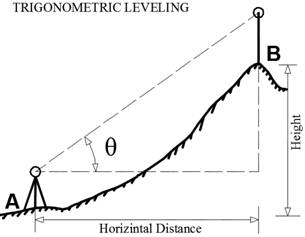
\includegraphics{"images/image010.jpg"}
\caption{ಟ್ರಿಗನಮಿಟ್ರಿಕಲ್​ ಲೆವಲಿಂಗ್}\label{chap6-fig1}
\end{figure}

ಆದರೆ, ಸ್ಪಿರಿಟ್​ ಲೆವೆಲಿಂಗ್​ ವಿಧಾನದಿಂದ ಎತ್ತರವನ್ನು ಅಳೆಯುವುದು, ಟ್ರಿಗನಮಿಟ್ರಿಕಲ್​ ವಿಧಾನಕ್ಕಿಂತ ಹೆಚ್ಚು ನಿಖರವಾದುದು ಮತ್ತು ಹೆಚ್ಚು ಸಮಯ ಹಿಡಿಯುವಂತಹದ್ದು. ಚಿತ್ರದಲ್ಲಿ ಸ್ಪಿರಿಟ್​ ಲೆವೆಲಿಂಗ್​ ವಿಧಾನವನ್ನು ನೋಡಬಹುದು.

\begin{figure}[!htbp]
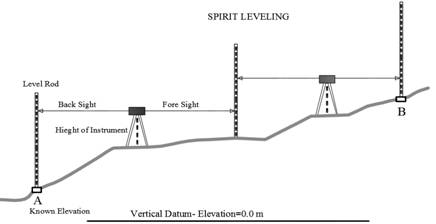
\includegraphics{"images/image011.jpg"}
\caption{ಸ್ಪಿರಿಟ್ ಲೆವಲಿಂಗ್}\label{chap6-fig2}
\end{figure}

ಲ್ಯಾಂಬ್​ಟನ್​ರವರ ಟ್ರಿಗನಮಿಟ್ರಿಕಲ್​ ಸರ್ವೇಗಿಂತ ಮೊದಲು ಇದ್ದಂತಹ ನಕ್ಷೆಗಳು, ಕೋಸ್ಟಲ್​ ಸರ್ವೇ ಮತ್ತು ಅಸ್ಟ್ರಾನಮಿಕಲ್​ ಸರ್ವೇ ಆಧಾರಿತ ನಕ್ಷೆಗಳು. ಅತ್ಯುತ್ತಮ ನಕ್ಷೆಗಳು ಎಂದೇ ಭಾವಿಸಲಾಗಿದ್ದ ನಕ್ಷೆಗಳು ಅವು. ಆ ಪ್ರಚಲಿತ ನಕ್ಷೆಗಳ ಪ್ರಕಾರ ಮದ್ರಾಸಿನಿಂದ ಮಂಗಳೂರವರೆಗಿನ ದೂರವು ಸುಮಾರು \enginline{400} ಮೈಲು ಇತ್ತು. ಆದರೆ, ಲ್ಯಾಂಬ್​ಟನ್​ರವರ ಟ್ರಿಗನಮಿಟ್ರಿಕಲ್​ ಸರ್ವೇಯಲ್ಲಿ ಆ ದೂರವನ್ನು \enginline{360} ಮೈಲು ಎಂದು ನಿರ್ಣಾಯಕವಾಗಿ ತೋರಿಸಲಾಯಿತು. ಟ್ರೈಯಾಂಗ್ಯುಲೇಷನ್​ ಸರ್ವೇಯ ಒಂದೇ ಹೊಡೆತಕ್ಕೆ \enginline{40} ಮೈಲುಗಳನ್ನು ತೆಗೆದುಹಾಕಬೇಕಾಯಿತು. ಇದು ಈ ಮೊದಲು ಇದ್ದ ಎಲ್ಲಾ ಸರ್ವೇ ಹಾಗೂ ಮ್ಯಾಪುಗಳು ದೋಷಯುತವಾಗಿರುವುದನ್ನು ತೋರಿಸಿತು. ಮತ್ತು ನಿಖರತೆಯ ಮ್ಯಾಪಿಗಾಗಿ\break ಟ್ರಿಗನಮಿಟ್ರಿಕಲ್​ ಸರ್ವೇಯ ಅಗತ್ಯವನ್ನು ಸಾರಿ ಹೇಳಿತು. ಸುಮಾರು \enginline{400} ಮೈಲುಗಳ ಅಗಲದ ಭೂ ಭಾಗವನ್ನು \enginline{360} ಮೈಲುಗಳಿಗೆ ಸೀಮಿತಗೊಳಿಸುವ ಅಳತೆ ಕಾರ್ಯ ಮಾತ್ರ ಯಾವುದೇ ಸರ್ಕಾರಕ್ಕೆ ಮಾಡುವ ಆಘಾತವೇ ಸರಿ. ಆದರೆ ಲ್ಯಾಂಬ್​ಟನ್​ರವರ ಟ್ರಿಗನಮಿಟ್ರಿಕಲ್​ ಸರ್ವೇಯು ಹೆಚ್ಚು ನಿಖರವಾದುದು. ಸರ್ವೇಯಲ್ಲಿ ನಿಖರತೆಗೇ ಮೊದಲ ಆದ್ಯತೆ.

\enginline{1806}ರಲ್ಲಿ ಪೂರ್ವದ ಮದ್ರಾಸ್​ ಮತ್ತು ಪಶ್ಚಿಮದ ಮಂಗಳೂರನ್ನು ಸಂಪರ್ಕಿಸಿದ ಅನಂತರ, ಲ್ಯಾಂಬ್​ಟನ್​ರವರು ಮುಂದಿನ ದಿನಗಳ ತಮ್ಮೆಲ್ಲಾ ಶ್ರಮವನ್ನು ಮೆರಿಡಿಯನಲ್​ ಆರ್ಕ್ ಅಳತೆಗೆ ಮುಡಿಪಾಗಿಟ್ಟರು. ಗ್ರೇಟ್​ ಆರ್ಕ್ ಕಾರ್ಯವನ್ನು ಬೆಂಗಳೂರು ಬೇಸ್​ಲೈನ್​\break ನಿಂದ ಉತ್ತರದ ಹಿಮಾಲಯದ ಕಡೆಗೂ ಮತ್ತು ದಕ್ಷಿಣದ ಕನ್ಯಾಕುಮಾರಿಯವರೆಗೂ ಮುಂದುವರೆಸಲಾಯಿತು. ಈ ಸರಣೀ ತ್ರಿಭುಜಗಳ ಮಹಾ ಪಟ್ಟಿಯನ್ನೇ ‘ಗ್ರೇಟ್​ ಆರ್ಕ್ ಸರಣಿ’ ಎನ್ನುವರು. ಮುಂದಿನ ಬೇಸ್​ಲೈನ್​ ಅಳತೆಯನ್ನು ಬೆಂಗಳೂರಿನಿಂದ \enginline{140} ಮೈಲು ದಕ್ಷಿಣಕ್ಕಿರುವ ಕೊಯಮತ್ತೂರು ಹತ್ತಿರ \enginline{1806}ರಲ್ಲಿ ಮಾಡಲಾಯಿತು. ಆರು ಮೈಲು ಉದ್ದದ ಬೇಸ್​ಲೈನ್​ನ ಟ್ರೈಯಾಂಗ್ಯುಲೇಷನ್​ ಮೌಲ್ಯಕ್ಕೂ, ನೆಲದ ಮೇಲಿನ ಅಳತೆಗೂ ಕೇವಲ \enginline{7.6} ಅಂಗುಲ ವ್ಯತ್ಯಾಸ ಬಂತು. \enginline{1808}ರಲ್ಲಿ ತಂಜಾವೂರು ಬೇಸ್​ಲೈನಿನ ಅಳತೆಯನ್ನು ಮಾಡಲಾಯಿತು.

